\documentclass[11pt]{article}

\usepackage{amsmath, amssymb, amsthm}
\usepackage{tikz}

\theoremstyle{plain}
\newtheorem{thm}{Theorem}[section]
\newtheorem*{thm*}{Theorem}
\newtheorem{prop}[thm]{Proposition}
\newtheorem{lem}[thm]{Lemma}
\newtheorem*{lem*}{Lemma}
\newtheorem{dfn}[thm]{Definition}
\newtheorem{cor}[thm]{Corollary}
\newtheorem{claim}[thm]{Claim}
\newtheorem{conj}[thm]{Conjecture}
\newtheorem{ques}[thm]{Question}
\newtheorem*{rem}{Remark}


\oddsidemargin  0pt
\evensidemargin 0pt
\marginparwidth 40pt
\marginparsep 10pt
\topmargin 0pt
\headsep 10pt
\textheight 8.2in
\textwidth 6.4in
\renewcommand{\baselinestretch}{1.1}

\newcommand{\codeg}{\text{codeg}}
\newcommand{\BBE}{\mathbb{E}}
\newcommand{\BFP}{\mathbf{P}}
\usepackage{amsmath}
\usepackage{amsthm}
\usepackage{amssymb}
\usepackage{mathtools}
\usepackage{hyperref}
\usepackage{url}





\usepackage{graphicx}
\usepackage{caption}
\usepackage{subcaption}

\def\eQb#1\eQe{\begin{eqnarray*}#1\end{eqnarray*}}
\def\eQnb#1\eQne{\begin{eqnarray}#1\end{eqnarray}}
\providecommand{\e}[1]{\ensuremath{\times 10^{#1}}}
\providecommand{\pb}[0]{\pagebreak}
\DeclarePairedDelimiter\ceil{\lceil}{\rceil}
\DeclarePairedDelimiter\floor{\lfloor}{\rfloor}

\newcommand{\E}{\mathrm{E}}
\newcommand{\Var}{\mathrm{Var}}
\newcommand{\Cov}{\mathrm{Cov}}

\def\Qb#1\Qe{\begin{question}#1\end{question}}
\def\Sb#1\Se{\begin{solution}#1\end{solution}}


\newtheoremstyle{quest}{\topsep}{\topsep}{}{}{\bfseries}{}{ }{\thmname{#1}\thmnote{ #3}.}
\theoremstyle{quest}
\newtheorem*{definition}{Definition}
\newtheorem*{theorem}{Theorem}
\newtheorem*{lemma}{Lemma}
\newtheorem*{question}{Question}
\newtheorem*{preposition}{Preposition}
\newtheorem*{exercise}{Exercise}
\newtheorem*{challengeproblem}{Challenge Problem}
\newtheorem*{solution}{Solution}
\newtheorem*{remark}{Remark}
\usepackage{verbatimbox}
\usepackage{listings}
\usepackage{mathrsfs}
\date{}
\title{\vspace{-0.7cm}
PDE II: Problem Set I}

\author{
Youngduck Choi 
\thanks{Department of Mathematics, Courant Institute of Mathematical Sciences, 
yc1104@nyu.edu; If you find an error and want to share with me, 
you can reach me via email.
}}

\begin{document}

\maketitle

\begin{abstract}
This work contains solutions for the problem set I.
\end{abstract}


\begin{question}[1-1]
\hfill
\begin{figure}[h!]
  \centering
    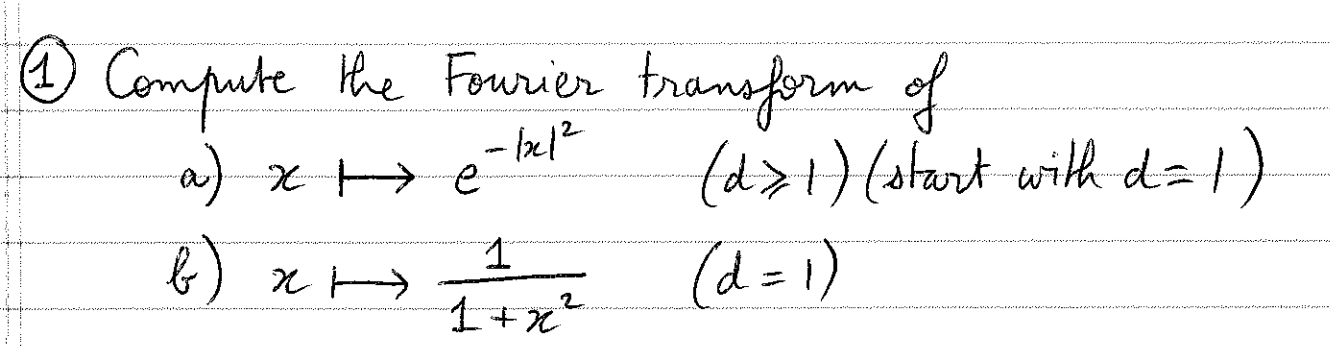
\includegraphics[width=0.7\textwidth]{pde2-1-1.png}
\end{figure}
\end{question}
\begin{solution} \hfill \\

\textbf{(a)} Set $u = x^2$ and $du = 2x dx$. Then,
\eQnb
\int_{-\infty}^{\infty} e^{-x^2} &=& \int_{0}^{\infty} u^{-\frac{1}{2}} e^{-u} du
= \Gamma(\dfrac{1}{2}). \label{eq:1-1-1}
\eQne
As
\eQb
\Gamma(1-s)\Gamma(s) &=& \dfrac{\pi}{\sin(\pi s)} 
\eQe
for any $s \in \mathbb{C}$, setting $s = \dfrac{1}{2}$ in the above and substituting
to~\eqref{eq:1-1-1} gives
\eQnb
\int_{-\infty}^{\infty} e^{-x^2} &=& \sqrt{\pi}. \label{eq:1-1-2}
\eQne
We now compute
\eQnb
\hat{f}(\xi) &=& \dfrac{1}{(2\pi)^{\frac{d}{2}}} \int_{\mathbb{R}^d} e^{-ix\cdot \xi}
e^{-|x|^2} \nonumber \\
&=& \dfrac{1}{(2\pi)^{\frac{d}{2}}} \prod_{k=1}^{d} \int_{\mathbb{R}} 
e^{-(x_k + \frac{i\xi_k}{2})^2 - \frac{\xi_k^2}{4}} dx_k \nonumber \\
&=& \dfrac{1}{(2\pi)^{\frac{d}{2}}} (\sqrt{\pi})^d e^{-\frac{|\xi|^2}{4}} 
\label{eq:1-1-3} \\ 
&=& 2^{-\frac{d}{2}}e^{-\frac{|xi|^2}{4}} \nonumber  
\eQne
for any $\xi \in \mathbb{R}^d$, where~\eqref{eq:1-1-3} follows from ~\eqref{eq:1-1-2}. 

\bigskip

\noindent 
\textbf{(b)} Firstly,
\eQnb
\hat{f}(\xi) &=& \dfrac{1}{\sqrt{2\pi}} \int_{\mathbb{R}} e^{-ix\xi} 
\dfrac{1}{1+x^2} dx \label{eq:1-2-1}
\eQne
for all $\xi \in \mathbb{R}$. Let $\xi < 0$. By Residue theroem,
\eQb
\int_{H + C_R} \dfrac{e^{-iz\xi}}{1+z^2} dz = 2\pi i \text{Res}(
\dfrac{e^{-iz\xi}}{1+z^2};i) = \pi e^{\xi}  
\eQe
for all $R > 0$ sufficiently large, where $C_R$ is the standard arc  and $H$
is the horizontal part of the upper half circle, oriented counter-clockwise. As
\eQb
\left| \int_{C_R} \dfrac{e^{-iz\xi}}{1+z^2} dz \right| &\leq& \dfrac{R}{R^2-1}
\int_{0}^{\pi} e^{R \xi \sin(\theta)} d\theta \leq \dfrac{\pi R}{R^2 -1} 
\eQe
for all $R > 0$, taking $R \to \infty$ gives
\eQb
\int_{\mathbb{R}} e^{-ix\xi} \dfrac{1}{1+x^2} dx &=& \pi e^{\xi}.
\eQe
Similarly, for $\xi \geq 0$, considering the lower half circle containing $-i$ gives
\eQb
\int_{\mathbb{R}} e^{-ix\xi} \dfrac{1}{1+x^2} dx &=& \pi e^{-\xi}
\eQe 
and hence, by~\eqref{eq:1-2-1},
\eQb
\hat{f}(\xi) &=& \sqrt{\dfrac{\pi}{2}} e^{-|\xi|} 
\eQe 
for all $\xi \in \mathbb{R}$. 
 
\end{solution}

\newpage

\begin{question}[1-2]
\hfill
\begin{figure}[h!]
  \centering
    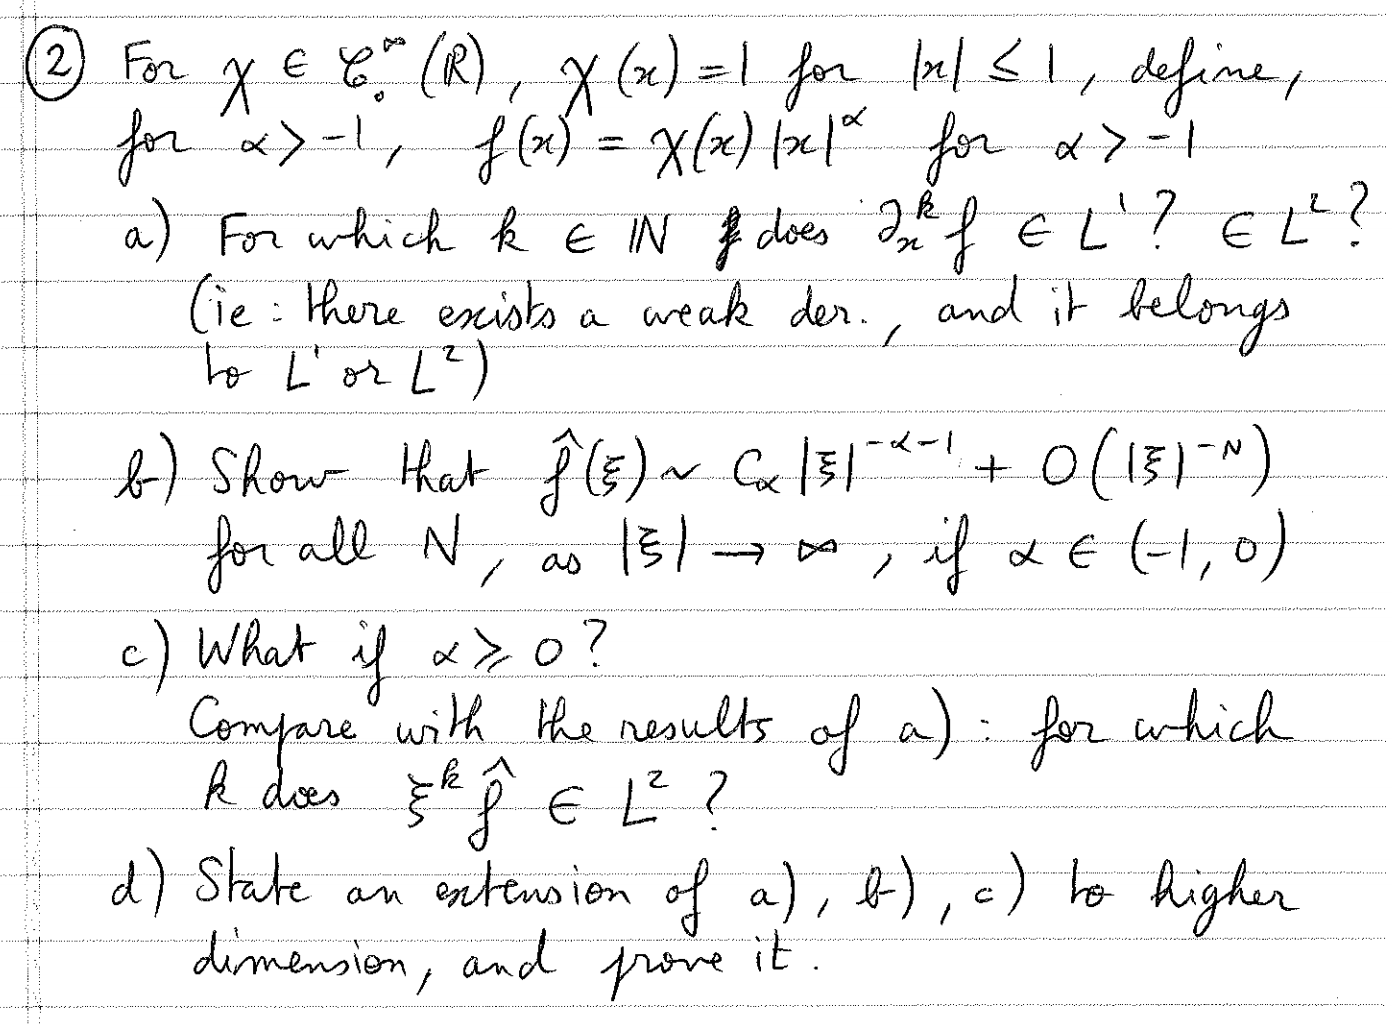
\includegraphics[width=0.7\textwidth]{pde2-1-2.png}
\end{figure}
\end{question}
\begin{solution} \hfill \\
ddd
\end{solution}

\newpage

\begin{question}[1-3]
\hfill
\begin{figure}[h!]
  \centering
    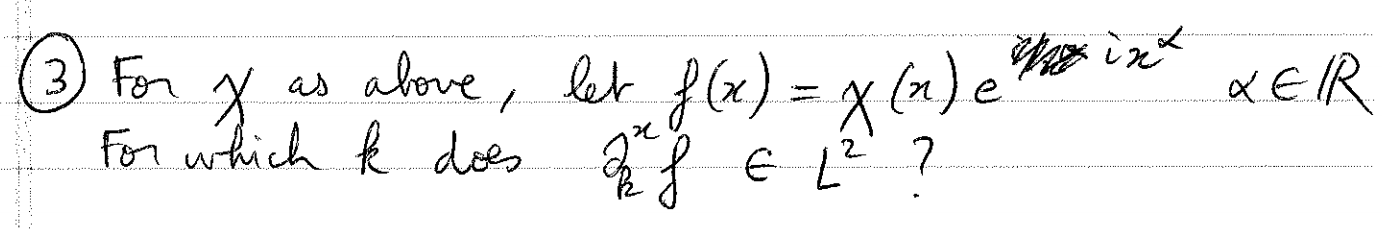
\includegraphics[width=0.7\textwidth]{pde2-1-3.png}
\end{figure}
\end{question}
\begin{solution} \hfill \\
ddd
\end{solution}

\newpage

\begin{question}[1-4]
\hfill
\begin{figure}[h!]
  \centering
    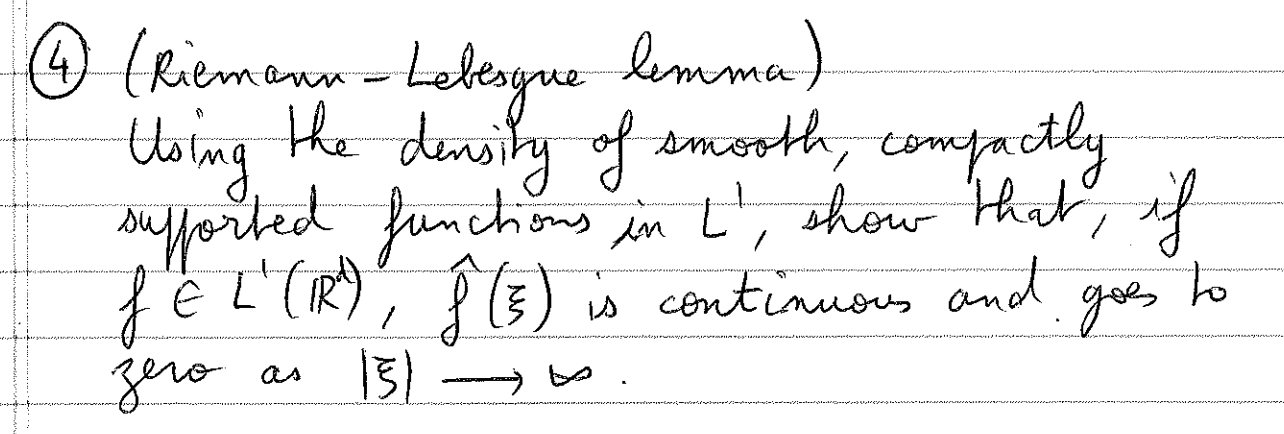
\includegraphics[width=0.7\textwidth]{pde2-1-4.png}
\end{figure}
\end{question}
\begin{solution} \hfill \\
The key property in this problem is that smooth and compactly supported functions
on $\mathbb{R}^d$ are dense in $L^1(\mathbb{R}^d)$, and $L^1$ convergence gives
uniform control on the Fourier domain.

Let $f \in L^1(\mathbb{R}^d), \xi \in \mathbb{R}^d$. Then, 
\eQb
|\hat{f}(\xi + \delta) - \hat{f}(\xi)| &=& \left|
\dfrac{1}{(2\pi)^{\frac{d}{2}}} \int_{\mathbb{R}^d} e^{-i x \cdot (\xi+\delta) } 
f(x) dx-
\dfrac{1}{(2\pi)^{\frac{d}{2}}} \int_{\mathbb{R}^{d}}  e^{-i x \cdot \xi} f(x) dx \right|
\\
&\leq& \dfrac{1}{(2\pi)^{\frac{d}{2}}} \int_{\mathbb{R}^d} |f(x)||e^{-ix \cdot 
(\xi+\delta)} - e^{-ix \cdot \xi}| dx \\
&\leq& \dfrac{1}{(2\pi)^{\frac{d}{2}}} \int_{\mathbb{R}^d} 2f(x) dx \in 
L^1(\mathbb{R}^d) 
\eQe
for all $\delta \in \mathbb{R}^d$. As 
\eQb
|e^{-ix \cdot (\xi + \delta)} - e^{-ix \cdot \xi} | \to 0 \>\>\> \text{as} 
\>\>\> \delta \to 0
\eQe
for all $x \in \mathbb{R}^d$, by DCT,
\eQb
\dfrac{1}{(2\pi)^{\frac{d}{2}}} \int_{\mathbb{R}^d} |f(x)||e^{-ix \cdot 
(\xi+\delta)} - e^{-ix \cdot \xi}| dx \to 0 \>\>\> \text{as} \>\>\> \delta \to 0 \\
\eQe
and hence, 
\eQb
\lim_{\delta \to 0} \hat{f}(\xi + \delta) - \hat{f}(\xi) &=& 0, 
\eQe
which shows that $\hat{f}$ is continuous.

\smallskip

\noindent Let $f \in C_{0}^{\infty}(\mathbb{R}^d)$. Then, 
\eQb
|\hat{f}(\xi)| &=& \left| \dfrac{1}{{(2\pi)}^{\frac{d}{2}}} 
\int_{\mathbb{R}^d}e^{-ix\cdot \xi} f(x) dx 
\right| \\
\eQe 
Therefore, the Riemann-Lebesgue lemma is true for $f \in C_{0}^{\infty}(\mathbb{R}^d)$.
Now, suppose $f \in L^1(\mathbb{R}^d)$. Then, by density of $C_0^{\infty}(\mathbb{R}^d)$
in $L^1(\mathbb{R}^d)$, 
we can choose $\{f_n\}_{n \in \mathbb{N}} 
\subset C_0^{\infty}(\mathbb{R}^d)$ such that $f_n \to_{L^1} f$ as $n \to \infty$.
Then,
\eQb
|\hat{f}(\xi) - \hat{f_n}(\xi)| &=& dd 
\eQe

\end{solution}

\newpage

\begin{question}[1-5]
\hfill
\begin{figure}[h!]
  \centering
    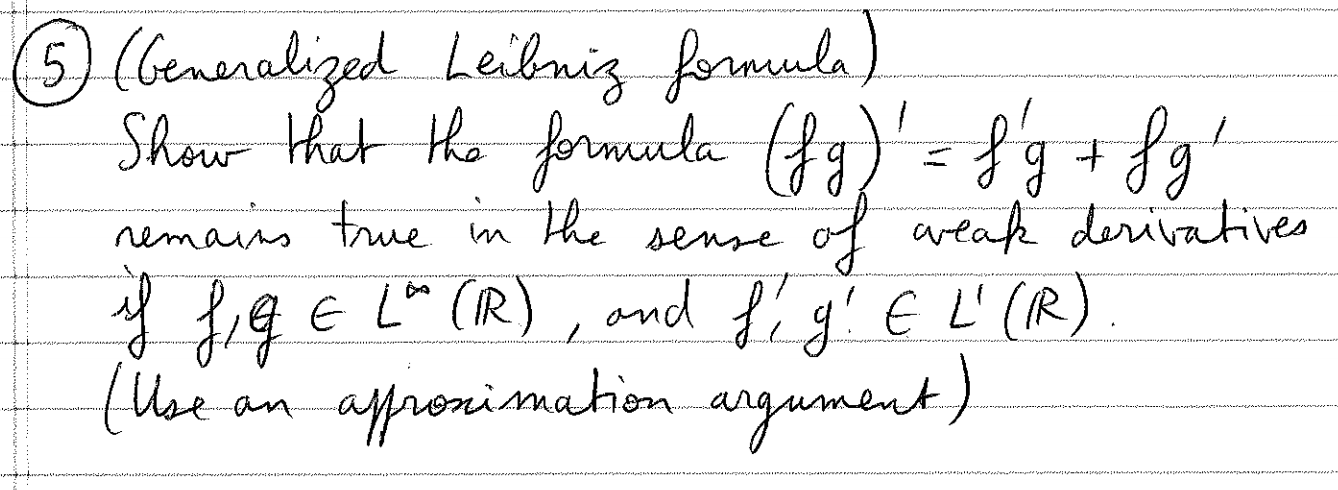
\includegraphics[width=0.7\textwidth]{pde2-1-5.png}
\end{figure}
\end{question}
\begin{solution} \hfill \\
We have
\eQb
\int_{\mathbb{R}} f\phi^{'} dx &=& - \int_{\mathbb{R}} f^{'} \phi dx 
\eQe
and
\eQb
\int_{\mathbb{R}} g\phi^{'} dx &=& - \int_{\mathbb{R}} g^{'} \phi dx
\eQe
for any $\phi \in \mathscr{S}$. We wish to show that
\eQb
\int_{\mathbb{R}} (fg) \phi^{'} dx &=& \int_{\mathbb{R}} (f'g + fg') \phi dx 
\eQe 
for any $\phi in \mathscr{S}$. 

\end{solution}


\end{document}
